\section{ХОД РАБОТЫ}

\subsection{Формулировка задачи}

Написать функцию для моделирования состояний цепи Маркова.
Входными параметрами этой функции выбрать вектор состояний, 
вектор начальных вероятностей, матрицу вероятностей перехода и
число шагов (тактов).

Использовать эту функцию для моделирования реализации состояний длительностью 
50 -- 100 тактов.
Реализацию вывести в графическом окне в виде графика.

Начальное состояние моделируется с использованием вектора
вероятностей начального состояния $ A $, а последующие --- с использованием 
соответствующих векторов-строк матрицы вероятностей перехода~$ P $.

Исходные данные: 
\begin{equation*}
P = \begin{pmatrix}
      0{,}6 & 0 & 0{,}4 \\
      0{,}4 & 0{,}6 & 0 \\
      0{,}4 & 0{,}2 & 0{,}4 \\
    \end{pmatrix},                            
A = \begin{pmatrix}
      0{,}3 & 0{,}7 & 0
    \end{pmatrix},
E = \begin{pmatrix}
      5 & 6 & 7
    \end{pmatrix}.
\end{equation*}


\subsection{Теоретические сведения}

\pagebreak

\subsection{Ход работы}

Исходный код разработанной программы представлен в приложении~А.

Полученные графики приведены на рисунке~\ref{pic:chain}.
\begin{figure}[h]
  \centering
  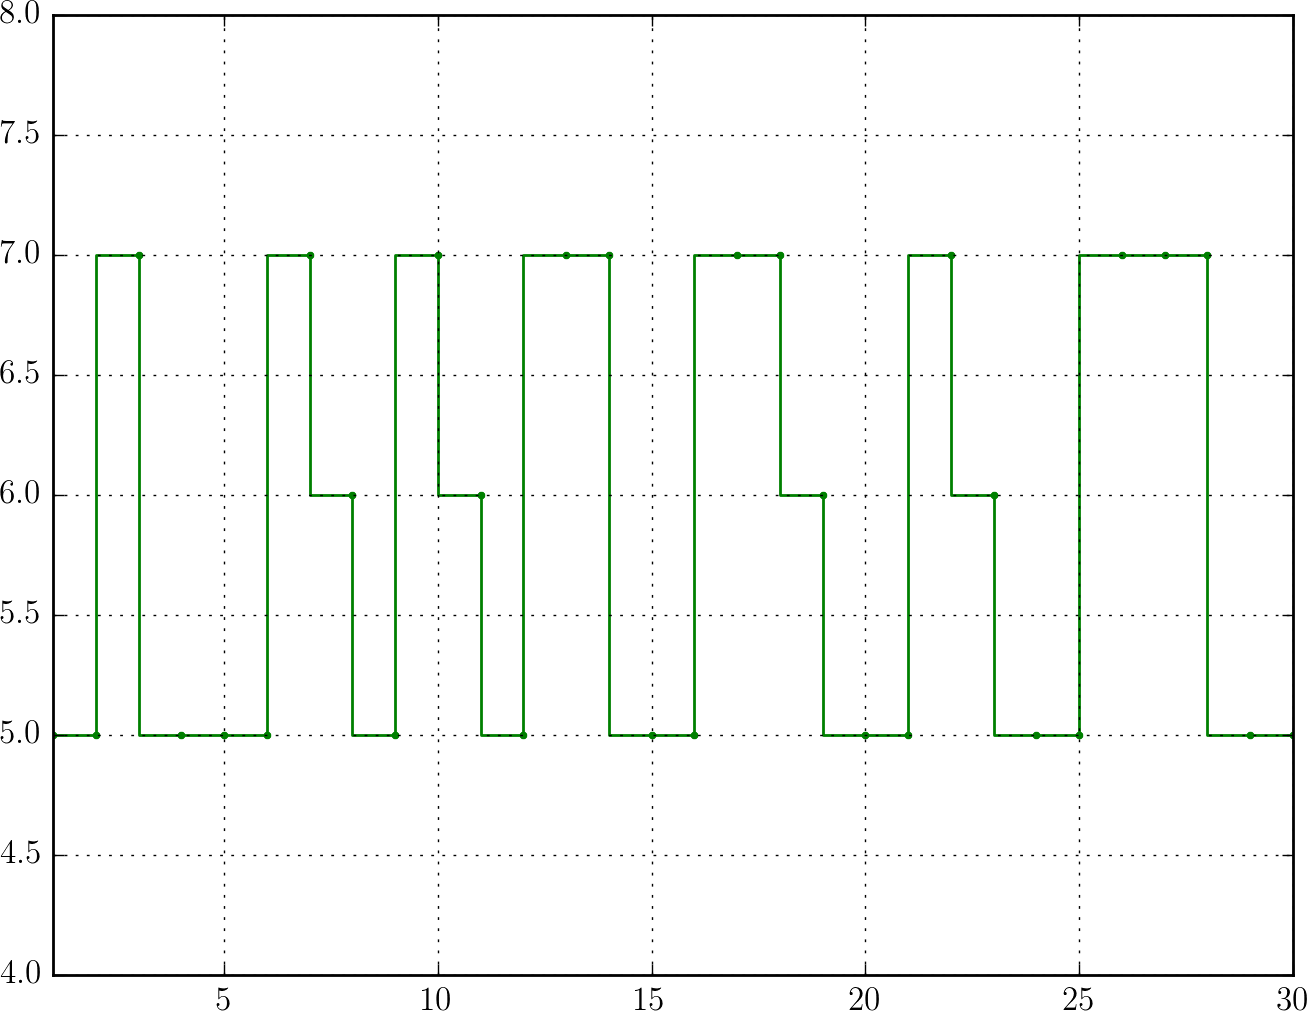
\includegraphics[width=150mm, height=92mm]{pic/chain}
  \caption{Последовательность случайных состояний, 
    подчиненных Марковской зависимости}
  \label{pic:chain} 
\end{figure}

\pagebreak